\chapter{说明}

\section{文件结构}

\texttt{figs}用于存放图片,\texttt{configuration}用于存放字体文件以及各种配置文件:
\begin{itemize}
    \item \texttt{CDUTReport.cls}: 调用宏包以及文档格式设置等
    \item \texttt{Font\_set.tex}: 字体设置.
    \item \texttt{Mycommand.sty}: 自定义命令,可以定义数学符号等.
    \item \texttt{Title\_set.tex}: 章节标题字体和格式的设置.
\end{itemize}
\texttt{ref.bib}为管理参考文献的文件;\texttt{titlepage.tex}为封面;\texttt{backpage.tex}为封底,用于填写实习心得。封面内容请在\texttt{main.tex}文件中编辑.


\section{插入公式}
插入行间公式,如式\ref{eq:1.1}
\begin{equation}
    \int_{a}^{b} f(x) \dl x = \lim_{\lambda(P) \to 0} \sum_{i=1}^n f(\xi_i) \Delta x_i  \label{eq:1.1}
\end{equation}
插入行内公式$\dim V = \dim \nul T + \dim \range T$.

矢量和矩阵一般写为粗体, 写法为$\bm{A} + \bm{B} = \bm{B} + \bm{A}$.

\section{插入图片}
\begin{figure}[H]
    \centering
    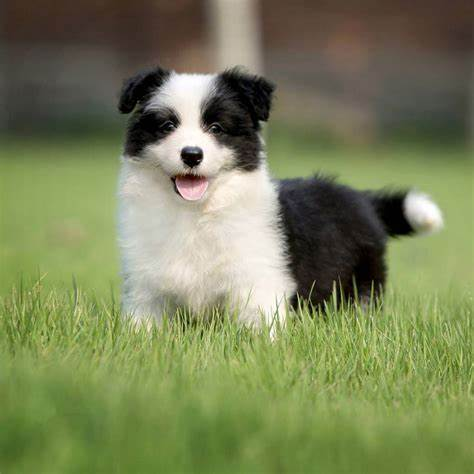
\includegraphics[width=3in]{figs/fig0.jpeg}
    \caption{边境牧羊犬又名边境柯利犬,是一种非常聪明的犬种,主要分布在四个国家——英国、美国、澳大利亚和新西兰。}
    \label{fig: 1}
\end{figure}

\section{插入表格} 

\begin{table}[H]
    \centering
    \caption{名字表}
    \label{table: 1}
    \begin{tabular}{ccc}
        \hline
        名字 & 年龄 & 专业 \\
        \hline
        \textbf{小王} & $20$ & 国际关系 \\
        \textbf{小美} & $22$ & 地球物理\\
        \textbf{小张} & $19$ & 软件工程 \\
        \hline
    \end{tabular}
\end{table}

\section{插入伪代码}

\begin{spacing}{1.0}  % 设置为原始行距使可以其紧凑一些
    \begin{algorithm}[H]
        \SetAlgoLined
        \KwData{单位法向量集$N=\{\bm{n}_i\}$, 太阳光矢量$\bm{l}$, 观察者矢量$\bm{e}$, 接收角度阈值$\theta_0$}
        \KwResult{接收光线数量$s$}
        $s \leftarrow 0$ \;
        \For{$\bm{n}_i$ in $N$}{
            \If{$\langle \bm{n}_i, \bm{l} \rangle \leq 0$}{
                $\bm{r}_i \leftarrow $ 根据$\bm{n}_i$随机生成单位反射矢量\;
                \If{$\langle \bm{r}_i, \bm{e} \rangle \geq \cos \theta_0$}{
                    $s \leftarrow s+1$\;
                }
            }
        }
        \caption{一次反射的模拟算法}
    \end{algorithm}
\end{spacing}

\section{粘贴代码}
请在\texttt{CDUTReport.cls}的\texttt{listings}设置中修改您的编程语言和代码高亮等内容。
\begin{spacing}{1.0}
\begin{lstlisting}
class Utils:
    @classmethod
    def mk_dir(cls, path):
        if os.path.exists(path):
            pass
        else:
            os.makedirs(path)
\end{lstlisting}
\end{spacing}

\section{引用}
由式\ref{eq:1.1}得。图\ref{fig: 1}展示了。表\ref{table: 1}中。参见\cite{Landou},参见\cite{liu-meng-2014-seemgo}


\section{字体}
本模板内置了{\heiti 黑体}, {\bfseries\heiti 粗黑体}, {\kaishu 楷书}, {\bfseries\songti 粗宋体}


\section{添加脚注并设置链接}

比如ESA用于发布詹姆斯韦伯望远镜照片的页面\footnote{\url{https://esawebb.org/images/}}.